Bigarren zati honetan, robotak \texttt{yahboom\_track} zirkuituari jarraitu behar dio kanpoaldetik, aurreko kamera erabiliz. Enuntziatuak eskatzen duen bezala, irudiaren prozesamendurako eta abiadurak kontrolatzeko hartu ditugun erabakiak arrazoitzen ditugu, eta lortutako emaitzak eztabaidatzen.

\section{Estrategia}\label{sec:er-estrategia}

\subsection{Sarrerako irudia}

\texttt{road\_perception} nodoak kameraren irudia segmentatzen du, eta emaitza \texttt{/road\_perception/ground} topic-ean argitaratzen du: $320 \times 240$ pixeleko gris-eskalako irudia, non 255 balioak errepidea adierazten duen (zuria) eta 0 balioak gainerakoa (beltza). Simulazioan, hormak eta bloke berdeak beltzez ageri dira; \egiaztatu{marra horiak eta oinezkoen pasabideak, berriz, errepidetzat hartzen dira}. \ref{fig:maskara}.~irudian, zirkuituaren hasieran jasotzen den irudiaren eskema ikus daiteke.

\begin{figure}[htbp]
  \centering
  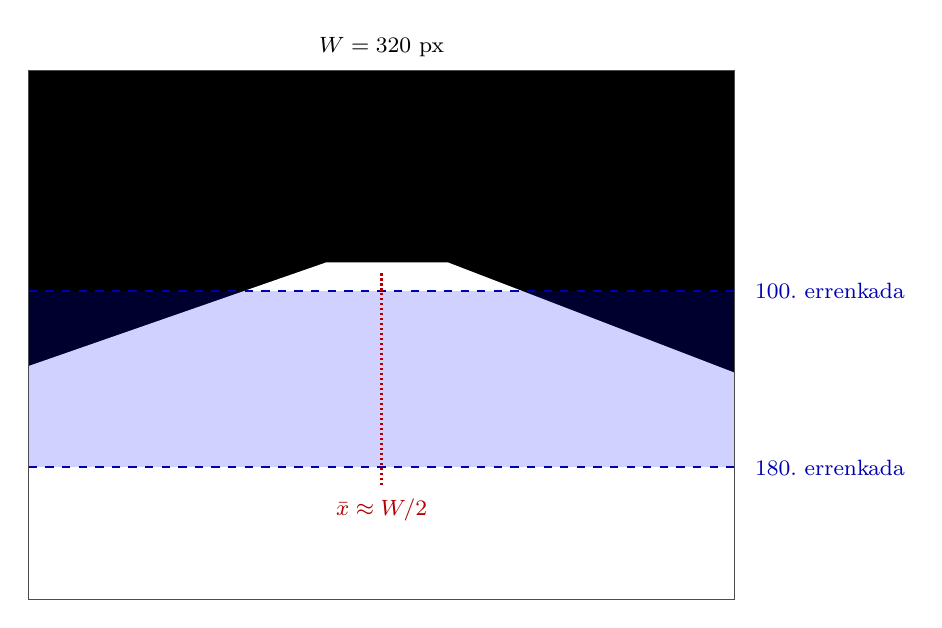
\begin{tikzpicture}[x=0.028cm, y=-0.028cm]
    \fill[black] (0,0) rectangle (320,240);
    \fill[white] (0,134) -- (135,87) -- (190,87) -- (320,137) -- (320,240) -- (0,240) -- cycle;
    \fill[blue, opacity=0.18] (0,100) rectangle (320,180);
    \draw[blue!70!black, thick, dashed] (0,100) -- (320,100) (0,180) -- (320,180);
    \draw[gray!60!black] (0,0) rectangle (320,240);
    \draw[red!70!black, thick, densely dotted] (160,92) -- (160,188);
    \node[red!70!black, font=\footnotesize, anchor=north] at (160,190) {$\bar{x} \approx W/2$};
    \node[blue!70!black, font=\footnotesize, anchor=west] at (325,100) {100.\ errenkada};
    \node[blue!70!black, font=\footnotesize, anchor=west] at (325,180) {180.\ errenkada};
    \node[font=\footnotesize, anchor=south] at (160,-2) {$W = 320$ px};
  \end{tikzpicture}
  \caption{Irudi segmentatuaren eskema, zirkuituaren hasieran jasotako irudian oinarritua. Errepidea zuriz ageri da; urdinez, zentroidea kalkulatzeko erabiltzen den banda. Zuzengune batean, $\bar{x} \approx W/2$ eta $e \approx 0$.}
  \label{fig:maskara}
\end{figure}

\subsection{Irudiaren prozesamendua}

Errepidearen norabidea jakiteko, errepide-pixelen \textbf{zentroidea} kalkulatzen dugu, hau da, pixel zurien zutabeen batez bestekoa, $\bar{x}$. Errepidea zuzen badoa, zentroidea irudiaren erdian geratzen da; eskuinerantz okertzen bada, eskuinera mugitzen da, eta alderantziz. Errorea zentroidea irudiaren erditik zenbat urruntzen den da, $-1$ eta $1$ artean normalizatuta:
\begin{equation}
  e = \frac{\bar{x} - W/2}{W/2}, \qquad W = 320.
\end{equation}

Ez dugu irudi osoa erabiltzen, \textbf{100. eta 180. errenkaden arteko banda} baizik. Erabaki hori robotak jasotzen duen irudiari begira hartu dugu:
\begin{itemize}
  \item 90. errenkada inguratik gora, irudia beltza da gehienetan (urrutiko hormak). Beraz, bandaren goiko muga gorago jarrita ere, ez da informazio gehiagorik lortzen.
  \item Beheko errenkadetan, errepideak irudiaren zabalera osoa betetzen du: robotaren ondoan, kameraren ikus-eremua estua da eta errepidea baino ez du ikusten. Errenkada horiek zentroidea erdirantz erakartzen dute eta erreakzioa moteltzen dute; 180. errenkadatik behera mozteak ez du informaziorik galtzen.
  \item Lehenengo bertsioetan banda estuago eta altuago bat erabiltzen genuen (96.--132.~errenkadak), eta robotak ez zuen zirkuitua osatzen \bete{zehaztu nola huts egiten zuen Gazebon}. Gure azalpena da banda horrek urrunegi begiratzen duela: robotak bihurgunea goizegi ikusten du, eta barruko blokea alboan duela hasten da biratzen.
\end{itemize}

Bandan errepide-pixelik ez badago (adibidez, horma bat aurrean duenean), robota gelditu eta eskuinera biratzen da, $\omega = -0{,}5$~rad/s abiaduran. Zirkuitua \egiaztatu{erlojuaren orratzen noranzkoan} egiten dugunez, barrualdea eskuinean dago, eta hara jotzen du errepideak bihurgune guztietan.

\subsection{Abiaduren kalkulua}

Biraketa-abiadura errorearekiko proportzionala da, eta abiadura lineala errorea handitu ahala txikitzen da:
\begin{equation}
  \omega = -K\,e, \qquad v = v_{\max}\,(1 - |e|).
\end{equation}
Minus zeinua ROSen hitzarmenagatik dago: $\omega > 0$ ezkerrera biratzea da; errepidea eskuinerantz badoa ($e > 0$), beraz, $\omega$ negatiboa izan behar da. Abiadura linealaren formulak robota moteltzen du bihurguneetan, biratzeko denbora izan dezan, eta zuzenguneetan abiadura maximoan joatea uzten dio. Txantiloiak, gainera, abiadurak mugatzen ditu: $v \le 0{,}3$~m/s eta $|\omega| \le 0{,}5$~rad/s.

$K$ irabazia abiadura maximoarekiko proportzionala da: $K = 15\,v_{\max}$. Lehenengo $K = 2$ finkoa erabili genuen; robotak ondo hartzen zituen bihurguneak, baina beranduxe hasten zen biratzen. $K$ handituta, lehenago erreakzionatzen du. Irabazia abiadurari lotzeko arrazoia, berriz, geometrikoa da. Robotaren ibilbidearen kurbadura $\kappa = \omega / v$ da, eta $K = 15\,v_{\max}$ aukeratuta:
\begin{equation}
  \kappa = \frac{\omega}{v} = \frac{-15\,v_{\max}\,e}{v_{\max}\,(1-|e|)} = \frac{-15\,e}{1 - |e|}.
\end{equation}
Kurbadura ez dago $v_{\max}$-ren mende: errore berarekin, robotak ibilbide bera egiten du edozein abiaduratan. $K$ finko batekin, ordea, abiadura jaistean kurbadura handitu egingo litzateke, eta robotak gehiegi biratuko luke bihurguneetan. Horri esker, robot errealean abiadura jaistean ez dugu beste parametrorik doitu behar.

\section{Inplementazioa}

\ref{lst:road}.~kode-zatian dago \texttt{road\_following.py} fitxategian osatu dugun zatia. Parametroak (\texttt{V\_MAX} eta \texttt{K}) nodoaren eraikitzailean definitzen dira: $\texttt{V\_MAX} = \egiaztatu{0{,}2}$~m/s eta $\texttt{K} = 15 \cdot \texttt{V\_MAX}$. Kodea iruzkinez beteta dago, enuntziatuak eskatzen duen bezala.

\begin{lstlisting}[caption={\texttt{road\_following.py} fitxategian osatutako zatia.},label={lst:road}]
# ESTRATEGIA: robotak aurrean ikusten duen errepidearen erdigunerantz
# (zentroidera) biratzen du. Irudi segmentatuan 255 = errepidea (zuria)
# eta 0 = ez-errepidea (beltza: hormak eta bloke berdeak).

# 1. Irudiaren zati bat bakarrik erabili: 100-180 errenkadak.
#    - Goiko errenkadak (100 baino gorago) urrunegi daude: bihurguneak
#      goizegi ikusten dira eta robotak barruko blokearen kontra biratzen du.
#    - Beheko errenkadak (180 baino beherago) errepidez beteta daude beti
#      (zabalera osoan zuriak) eta ez dute informaziorik ematen.
zatia = cv_image[100:180, :]

# 2. Errepideko pixel guztien posizioak lortu (255 = errepidea).
#    'zutabeak' pixel zuri bakoitzaren zutabea da (0 ezkerrean, 319 eskuinean).
errenkadak, zutabeak = np.nonzero(zatia > 127)

if len(zutabeak) == 0:
    # 3a. Errepiderik ez da ikusten (adib. horma bat aurrean):
    #     gelditu eta eskuinera biratu, zirkuituaren barrualdera.
    linear_velocity = 0.0
    angular_velocity = -0.5
else:
    # 3b. Errepidearen erdigunea: pixel zurien zutabeen batez bestekoa.
    erdigunea = np.mean(zutabeak)

    # 4. Errorea: erdigunea irudiaren erditik zenbat urruntzen den,
    #    -1 (guztiz ezkerrean) eta 1 (guztiz eskuinean) artean.
    #    error > 0 -> errepidea eskuinerantz doa (adib. eskuineko bihurgunea)
    #    error < 0 -> errepidea ezkerrerantz doa
    error = (erdigunea - image_width / 2) / (image_width / 2)

    # 5. Kontrol proportzionala: errepidea dagoen aldera biratu.
    #    ROS-en angular.z > 0 ezkerrera da eta < 0 eskuinera; horregatik minus zeinua.
    angular_velocity = -self.K * error

    # 6. Abiadura lineala: zenbat eta errore handiagoa (bihurgunea),
    #    orduan eta motelago, biratzeko denbora izateko.
    linear_velocity = self.V_MAX * (1 - abs(error))
\end{lstlisting}

\section{Simulazioko ebaluazioa}

\texttt{yahboom\_track} munduan, robotak \bete{N}~bira oso eman ditu $v_{\max} = \egiaztatu{0{,}2}$~m/s-rekin, eta bira bakoitzak \bete{T}~s inguru iraun du. \bete{Deskribatu portaera: zuzenguneetan egonkor doa? Nola hartzen ditu bihurguneak? Bidegurutzeetan barrura sartzen da?}

Zentroidea erabiltzeak arrisku bat du bidegurutzeetan: barruko kale batek errepidea alde batera zabaltzen duenean, zentroidea harantz mugitzen da, eta robota kale horretara desbidera daiteke. \bete{Gure probetan, \ldots}. Gure azalpena da irekiera bandaren zati txiki batean eta denbora laburrean agertzen dela, eta, beraz, zentroidea apur bat baino ez duela mugitzen.

\section{Robot errealarekin egindako ebaluazioa}\label{sec:er-erreala}

\subsection{Abiaduren doikuntza}

Robot errealean, segmentazio-nodoa eskuz abiarazi behar da:
\begin{lstlisting}[language=bash, numbers=none]
ros2 launch road_perception road_segmentation_deeplabv3.launch.py
\end{lstlisting}
Abiadura maximoa \bete{0,1--0,15}~m/s-ra jaitsi dugu, \bete{arrazoiak: segmentazioaren atzerapena, irudi-maiztasuna, gurpilen eta lurraren portaera\ldots}. $K = 15\,v_{\max}$ denez, irabazia automatikoki egokitzen da, eta \egiaztatu{ez dugu beste parametrorik aldatu behar izan}.

\subsection{Emaitzak}

Enuntziatuak eskatzen duen bezala, zirkuituan bira osoa emateko bost saiakera egin ditugu (\ref{tab:saiakerak}.~taula). Arrakasta-ehunekoa osatutako biren proportzioa da, eta batez besteko denbora osatutako birekin bakarrik kalkulatu dugu.

\begin{table}[htbp]
  \centering
  \begin{tabularx}{\textwidth}{@{}>{\centering\arraybackslash}p{1.8cm}>{\centering\arraybackslash}p{3cm}>{\centering\arraybackslash}p{2.2cm}X@{}}
    \toprule
    Saiakera & Bira osatu du? & Denbora (s) & Oharrak \\
    \midrule
    1 &  &  &  \\
    2 &  &  &  \\
    3 &  &  &  \\
    4 &  &  &  \\
    5 &  &  &  \\
    \midrule
    \multicolumn{4}{@{}l}{Arrakasta-ehunekoa: \hspace{3em}\%\qquad Bira baten batez besteko denbora: \hspace{3em}s} \\
    \bottomrule
  \end{tabularx}
  \caption{Robot errealarekin egindako bost saiakeren emaitzak.}\label{tab:saiakerak}
\end{table}

\subsection{Eztabaida}

\bete{Zergatik huts egin dute huts egin duten saiakerek? Zer alde dago simulazioaren eta robot errealaren artean? Adibidez: argiztapena eta islak, segmentazio-akatsak, irudien atzerapena, gurpilen irristatzea.}

\section{Ondorio partzialak}

Estrategia sinple batekin (zentroidea eta kontrol proportzionala), robotak \bete{emaitza nagusia simulazioan eta robot errealean}. Erabakirik garrantzitsuena irudiaren banda aukeratzea izan da: urrunegi begiratuz gero, robotak bihurguneak goizegi hartzen ditu; hurbilegi begiratuz gero, berandu. Irabazia abiadurari lotzeak, berriz, simulaziotik robot errealera pasatzea erraztu digu. \bete{Hobekuntzak: adibidez, kanpoko ertzari zuzenean jarraitzea, bidegurutzeak hobeto kudeatzeko.}
